% NEEDS TO BE COMPILED WITH pdflatex

\documentclass[portrait,a0paper]{baposter}

\usepackage{graphicx}
\usepackage[utf8]{inputenc}
\usepackage{tabto}
\usepackage{booktabs}
\usepackage{amsmath}
\usepackage{float}
\usepackage{multirow}
\usepackage[hyphens]{url}
\usepackage{enumitem}
\usepackage{ragged2e}
\usepackage{qrcode}
\usepackage{textcomp}

\newlength{\mytextsize}
\setlength{\unitlength}{1.0cm}

%###########################################################################################################################
% Customize here ############################################################################################################

\def\posterTitle{%
    Data-driven low-code programming system
}
\def\posterAuthor{%
   Jaroslav Švarc 
}
\def\posterSchool{%
  Faculty of Mathematics and Physics, Charles University
    }
\def\posterYear{%
    2025
}
\def\posterLogoFaculty{logos/mff-white.pdf}
\def\posterLogoSchool{logos/uk-white.pdf}

\definecolor{maincolor}{RGB}{119, 221, 119}
\definecolor{headercolor}{RGB}{255,255,255}
\definecolor{textbackgroundcolor}{RGB}{255,255,255}
\definecolor{highlightcolor}{RGB}{70,150,255}
\colorlet{highlightbackgroundcolorOne}{red!60!orange!03}
\colorlet{highlightbackgroundcolorTwo}{red!60!orange!15}
\def\backgroundcolor{gray!25}

\usepackage[scaled]{helvet}
% Uncomment for non-serif text font
% \renewcommand*\familydefault{\sfdefault}

%###########################################################################################################################
% My own macros and commands ###############################################################################################

% Custom red markings for TODO items
\newcommand{\todo}[1]{%
    \textcolor{red}{\textbf{#1}}% Bold and red text
    \PackageWarning{TODO}{#1}% Warning in LaTeX log
}
% Custom headerbox command to left-align text
\newcommand{\leftalignedheaderbox}[3]{\headerbox{#1}{#2}{%
    % Uncomment for left-aligned text
    % \RaggedRight{%
    #3
    % }
}}
% Custom headerbox command with highlighted background
\newcommand{\highlightheaderbox}[3]{\leftalignedheaderbox{#1}{#2,%
boxColorOne=highlightbackgroundcolorOne,boxColorTwo=highlightbackgroundcolorTwo%
}{#3}}
% Custom headerbox without a header, intended for additional info at the bottom of the poster
\newcommand{\footerbox}[2]{\headerbox{}{#1,%
above=bottom,borderColor=maincolor,boxheaderheight=1pt%
}{#2}}
% Text highlighting
\newcommand{\highlight}[1]{\textbf{\color{highlightcolor}#1}}

%###########################################################################################################################
\begin{document}
\begin{poster}
	{
		grid=false, % Debugging or Layour grid
		eyecatcher=false, % Custom main header
		columns=6, % for flexibility -- changing 2/3 columns with columnspan
		%
		background=plain,
		bgColorOne=\backgroundcolor,
		%
		headerfont=\bf\Large\sffamily,
		headerFontColor=headercolor,
		headershape=rectangle,
		headershade=plain,
		headerColorOne=maincolor,
		headerborder=open,
		%
		boxshade=shadetb,
		boxColorOne=textbackgroundcolor,
		boxColorTwo=textbackgroundcolor,
		textborder=rectangle,
		borderColor=maincolor,
		boxpadding=1em
	}{}{
		% poster title
		\hspace*{-0.5mm}
		\begin{picture}(23.7, 3)
			\fboxsep0pt
			\put(-0.196, -0.6){\colorbox{maincolor}{\rule[96pt]{675.82pt}{0pt}}}
			\thicklines
			% minipage box for title and authors
			% Faculty logo
			\put(0.24,-0.24){\includegraphics[height=75pt]{\posterLogoFaculty}}
			\put(2.55, 2.35){
				\begin{minipage}[t][96pt]{0.75\textwidth}
					\begin{center}
						{\huge\bf\color{headercolor}\sffamily%
							\posterTitle \\[0.35cm]
						}
						{\large\color{headercolor}\sffamily%
							\posterAuthor
							\raisebox{0.1em}{$\bigm\lvert$}
							\posterSchool
							\raisebox{0.1em}{$\bigm\lvert$}
							\posterYear
							\\
						}
					\end{center}
				\end{minipage}}
			\put(20.52,-0.24){\includegraphics[height=75pt]{\posterLogoSchool}}
		\end{picture}
	}{}{}
	% ==========================================================================================================================
	% Footer ===================================================================================================================
	% Puting the footer first might seem counter-intuitive but trust me on this one.
	% In order to reference the footer elements for bottom-alignments, the footer boxes need to be defined first.
	\footerbox{%
		name=repository,column=2,span=4%
	}{
		\begin{minipage}{.17\textwidth}
			\begin{center}
				\qrcode[height=2cm]{https://github.com/JerrySvarc/InterfaceSmith}%
			\end{center}
		\end{minipage}%
		\begin{minipage}{.66\textwidth}
			\textbf{\large\sffamily\color{maincolor}Repository}
			\\[0.25em]
			\scriptsize\url{https://github.com/JerrySvarc/InterfaceSmith}
			% \vfill\hrule\vfill
			\vspace{0.55em}\hrule\vspace{0.55em}
			\hfill\textbf{\large\sffamily\color{maincolor}Thesis}
			\\[0.25em]
			\scriptsize\url{https://jerrysvarc.github.io/bachelor-thesis/thesis.pdf}
		\end{minipage}%
		\begin{minipage}{.17\textwidth}
			\begin{center}
				% If the thesis URL is short, I would right align it also: BTW I have no idead why the \phantom{a} helps,
				% but it helped me, so might aswell leave it for other unfortunate souls
				% \phantom{a}\hfill%
				\qrcode[height=2cm]{https://jerrysvarc.github.io/bachelor-thesis/thesis.pdf}%
			\end{center}
		\end{minipage}%
	}
	\footerbox{%
	name=supervisor,column=0,span=2,aligned=repository% Although this box is to the left of the aligning box,
	% and thus would be logical to define it first, the QR codes were messy when I worked on this template
	% so I leave the QR codes box to choose its height and then alighn this one next to it.
	}{
	% By all means, laugh away at the brutal by-hand vertical spacing...
	% But then also feel free to change it.
	\textbf{\sffamily\large\color{maincolor}Supervisor}
	\\[0.4em]
	{\large Mgr. Tomáš Petříček, Ph.D.}
	\\[0.1em]
	Department of Distributed and Dependable Systems
	}
	% ==========================================================================================================================
	\leftalignedheaderbox{Intro}{%
		name=intro,column=0,row=0,span=3% Note the `name` value, used later for layout definition
	}{
		Low-code programming systems provide a graphical user interface (GUI), through which users can create software elements.
		Software development using low-code programming systems is increasingly popular and
		traditional low-code development systems that provide user interface creation functionality primarily provide the \emph{UI-to-data} approach, where developers create user interface elements before populating them with data.
		However, the \emph{data-to-UI} approach, where the development process begins with concrete data that drives the creation of corresponding UI elements, remains unexplored as a primary development method.
		We present the InterfaceSmith prototype programming system, which implements \emph{data-to-UI} as the primary development method for creating web applications' UI elements.

		\begin{center}
			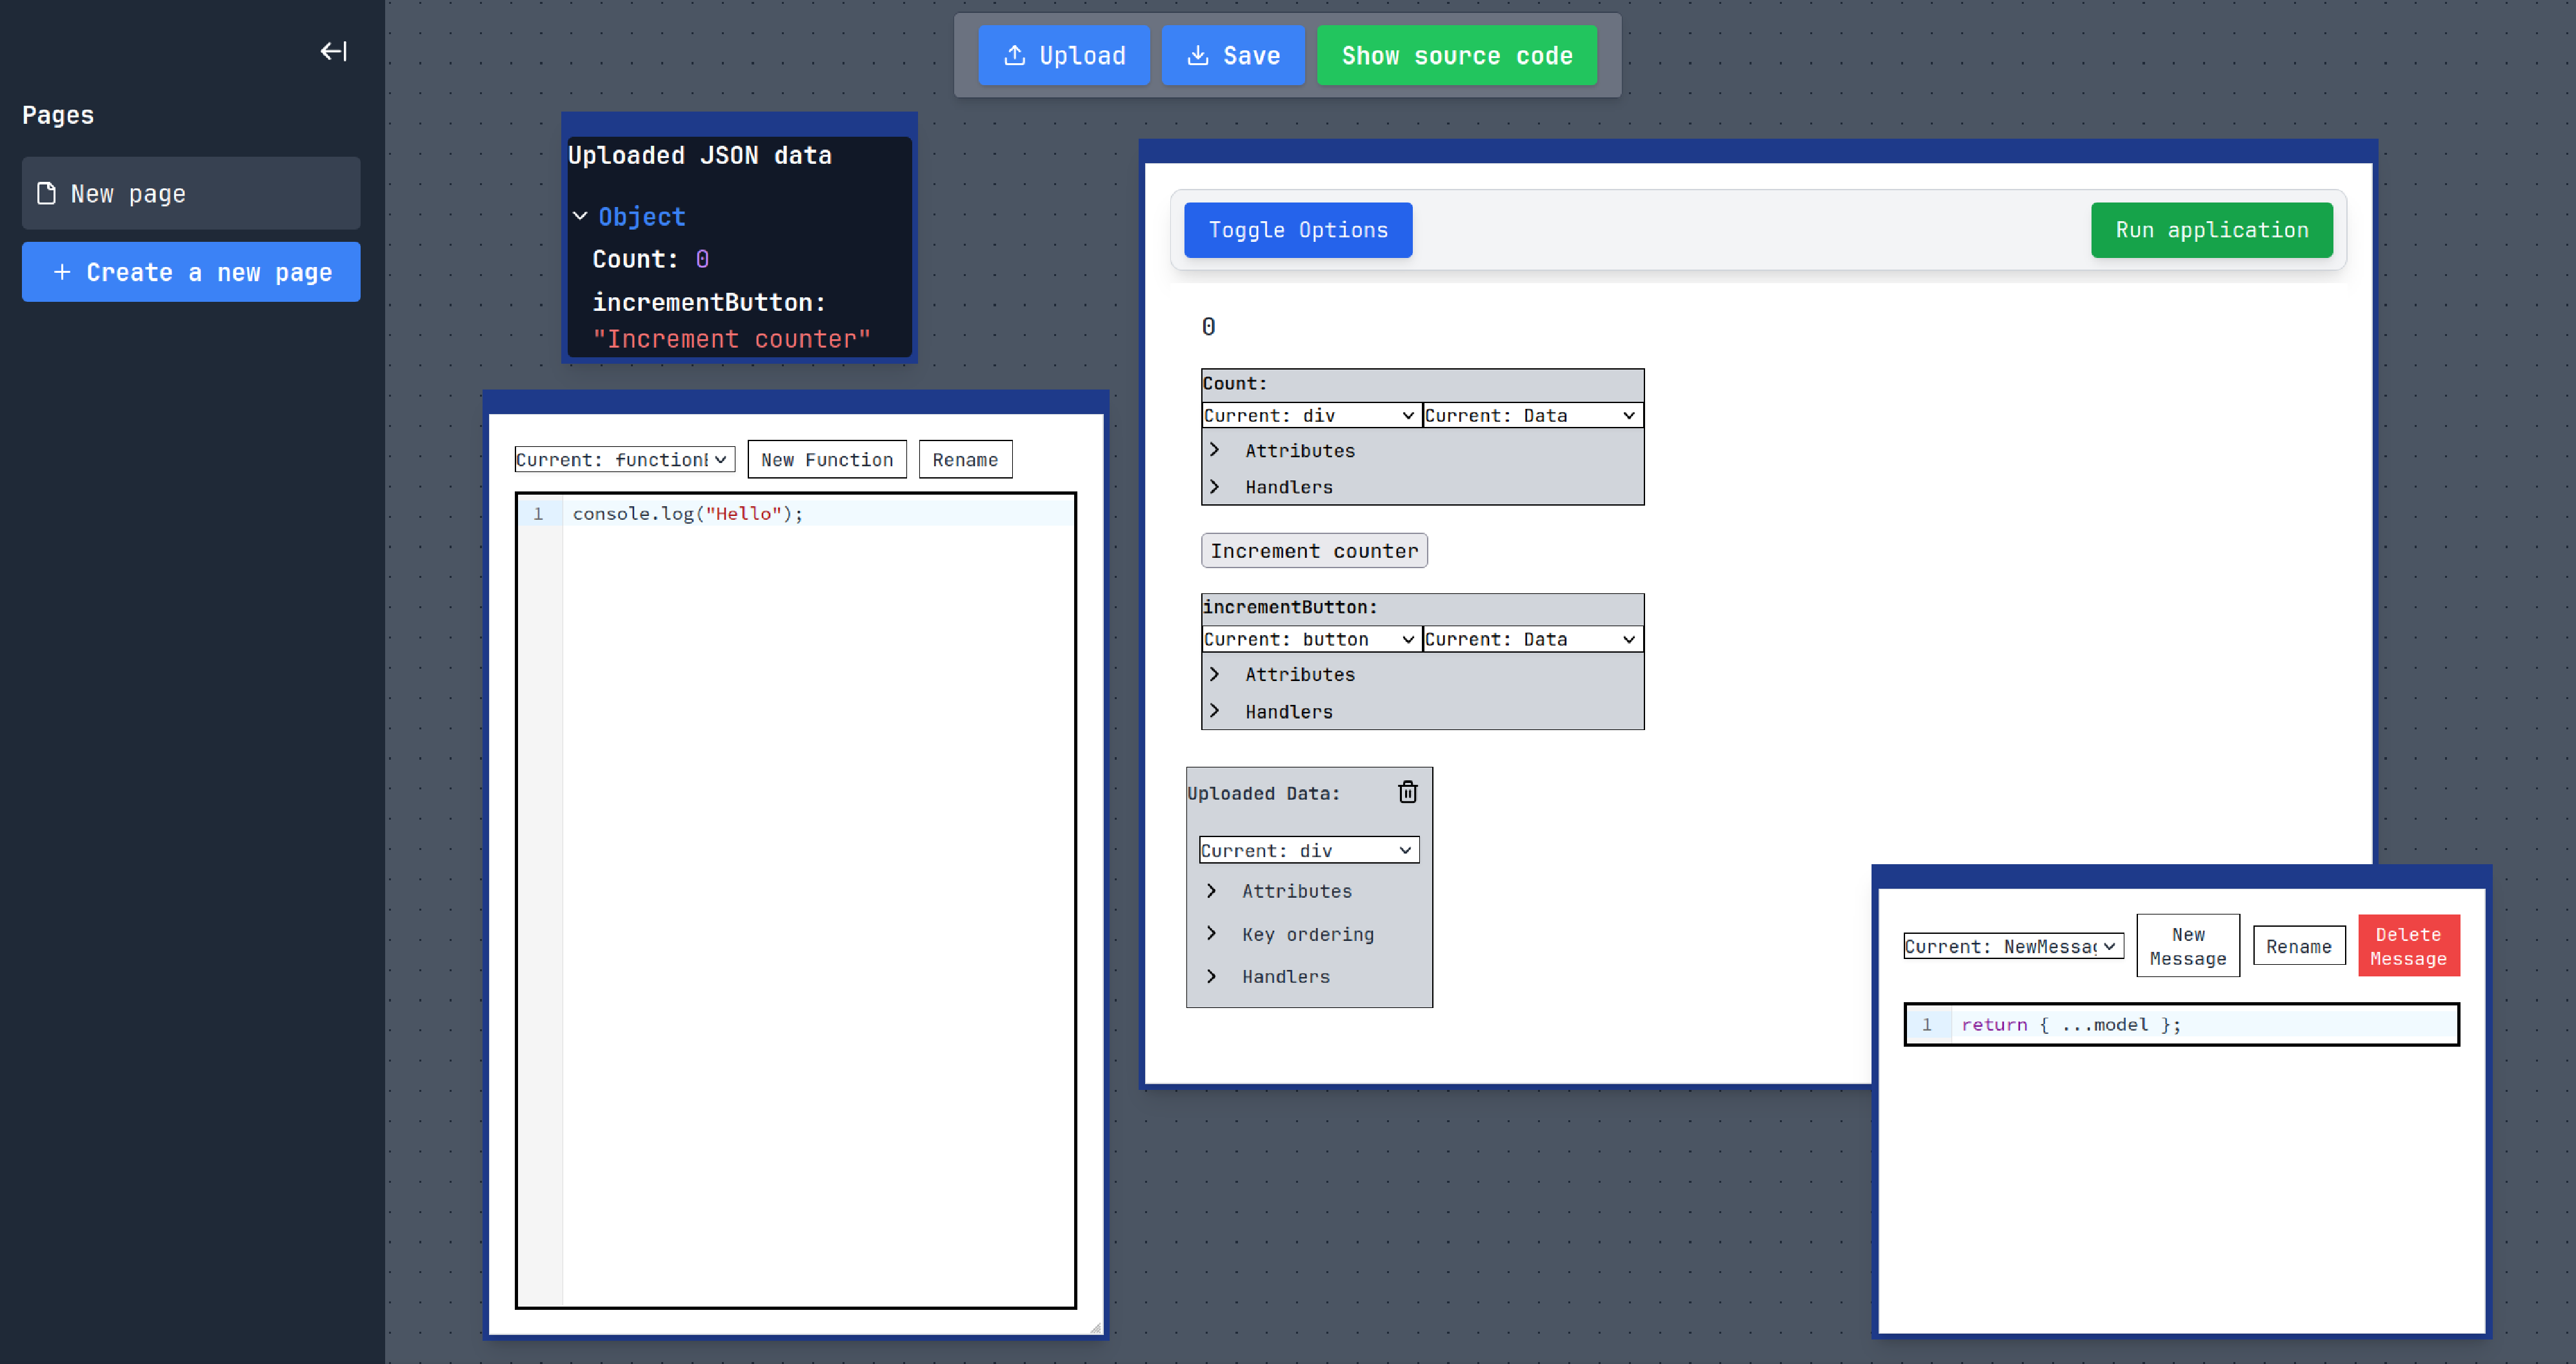
\includegraphics[width=0.95\textwidth]{img/UIExample.pdf}
		\end{center}

	}

	\leftalignedheaderbox{Motivation}{
		name=motivation,column=0,span=3,below=intro% Note how `aligned` defines that this box starts exactly with the specified box
	}{
		The primary motivation for this research is to allow the creation of single-page web applications following the Elm architecture, also known as Model-View-Update, based on concrete
		data uploaded to the system. The aim is to allow incremental creation of UI elements based on the uploaded data's type and structure.
	}

	% --------------------------------------------------------------------------------------------------------------------------
	\leftalignedheaderbox{Goals}{
		name=goals,column=0,span=3,below=motivation% Note how `below` defines that this box is exactly below the intro box
	}{
		\begin{enumerate} [leftmargin=*]
			\item Explore the
			\item Create a working \textbf{prototype programming system} implementing the data-driven approach.
			\item Benchmark the prototype application on the following tasks:
			      \begin{itemize}
				      \item A simple \textbf{TO-DO list} application inspired by the \emph{TodoMVC} becnhmark.
				      \item \textbf{Counter} task from the \emph{7GUIs} becnhmark.
				      \item \textbf{Temperature converter} task from the \emph{7GUIs} becnhmark.
			      \end{itemize}
		\end{enumerate}
	}
	% --------------------------------------------------------------------------------------------------------------------------

	% --------------------------------------------------------------------------------------------------------------------------
	\leftalignedheaderbox{Solution approach}{% Note how this box is highlighted
		name=solutionApproach,column=3,span=3
		% Note how `row` defines an arbitrary vertical placement in the layout
		% - see the `grid` option of the `poster` environment to enable the layout grid
		% Note how the combination of the `column` and `span` options places the box at a central position
		% However, for a "central result box" layout, I suggest changing the `columns` option of the `poster` environment
		% to a different value, allowing for better ratios between spanning columns.
	}{
		\todo{Hole-based approach, traversal, example image }
	}
	% --------------------------------------------------------------------------------------------------------------------------
	\leftalignedheaderbox{Experiments}{%
		name=ssira,column=3,span=3,below=solutionApproach % Note how `above` defines that this box ends exactly above the specified box
	}{

		\begin{tabular}{|p{3cm}|c|c|c|c|c|}
			\hline
			\textbf{Task}   & \textbf{Total} & \textbf{Prep} & \textbf{Custom} & \textbf{Ref.} & \textbf{Success} \\
			\hline
			TO-DO List      & 54             & 14            & 40              & N/A           & Yes              \\
			Counter         & 8              & 4             & 4               & 11            & Yes              \\
			Temp. Converter & 34             & 6             & 28              & 66            & Yes              \\
			\hline
		\end{tabular}

		\begin{tabular}{|p{2.5cm}|c|c|c|}
			\hline
			\textbf{Task}   & \textbf{Total} & \textbf{Data Prep (\%)} & \textbf{Custom Logic (\%)} \\
			\hline
			TO-DO List      & 54             & 26\%                    & 74\%                       \\
			Counter         & 8              & 50\%                    & 50\%                       \\
			Temp. Converter & 34             & 18\%                    & 82\%                       \\
			\hline
		\end{tabular}


	}
	% --------------------------------------------------------------------------------------------------------------------------
	\leftalignedheaderbox{Summary}{%
		name=summary,column=3,span=3,above=repository, below=ssira % Note how `bottomaligned` defines that this box ends exactly where the specified box ends
	}{


	}
\end{poster}
\end{document}
